\documentclass{beamer}
\usepackage{sansmathaccent}
\usepackage{gensymb}
\pdfmapfile{+sansmathaccent.map}
\usepackage{comment}
\usepackage{physics}
\usetheme{Madrid}

\usepackage[utf8]{inputenc}
\usepackage{graphicx}

\title[21 cm]{Determining Galactic Strucutre through 21cm Emission Lines}
\author{Henry Shackleton}

\begin{document}

\titlepage

\section{Introduction and Theory}

\begin{frame}
  \frametitle{Hyperfine Strucutre of Hydrogen Emits 21cm Wavelenth Emission}
  \begin{columns}
    \begin{column}{0.7\textwidth}
      \begin{center}
  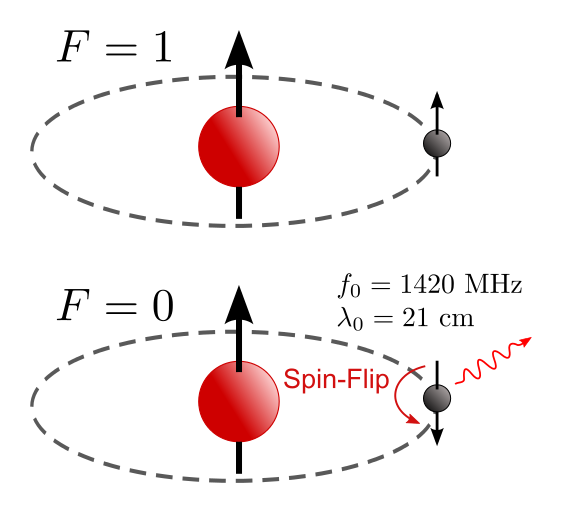
\includegraphics[width=0.7\linewidth]{hyperfine}
\end{center}
\end{column}
\begin{column}{0.3\textwidth}
  \begin{center}
    \begin{itemize}
      \item Hydrogen electron spin-flip causes electromagnetic radiation at a frequency of $1420.41$ MHz.
      \item Low probability ($2.9 \times 10^{-15} s^{-1}$), but the vast amount of hydrogen in the galaxy allows for this detection
    \end{itemize}\end{center}\end{column}\end{columns}
\end{frame}

\begin{frame}
  \frametitle{Doppler Shift Gives Change in 21cm Line Proportional to Velocity}
  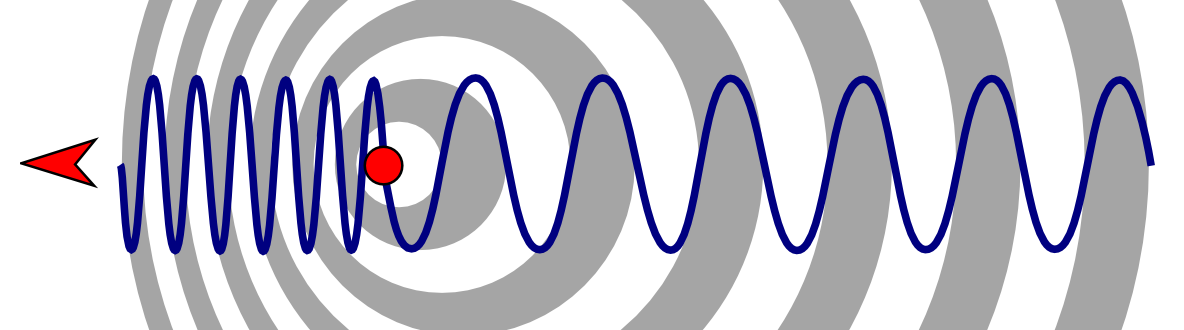
\includegraphics[width=1\textwidth]{diagrammatic}
  \begin{equation*}
  v = c \frac{1420.41 - \nu}{\nu}
\end{equation*}
\end{frame}

\begin{frame}
  \frametitle{Location of Hydrogen Masses Determined through Geometry}
  \begin{columns}
    \begin{column}{0.4\textwidth}
  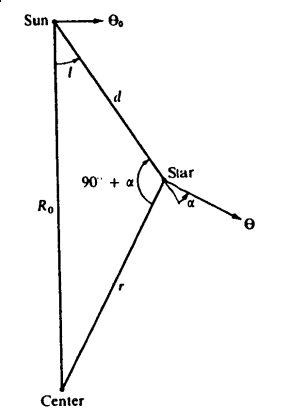
\includegraphics[width=1\textwidth]{geom}
\end{column}
\begin{column}{0.6\textwidth}
  \begin{itemize}
    \item Velocity we observe is the velocity of the mass \textit{projected} onto our line of sight. 
    \item $v_{obs} = \frac{\Theta}{r} R_0 \sin \ell - \Theta_0 \sin \ell$
    \item Relation between $\Theta$ and $r$ obtained through Galactic Rotation Curve.
    \item Between $90\degree < \ell < 180\degree$, Galactic Rotation Curve is approximately constant.
  \end{itemize} 
\end{column}
\end{columns}
\end{frame}

\begin{frame}
  \frametitle{SRT Measures Radio Power Within Given Frequency Domain}
  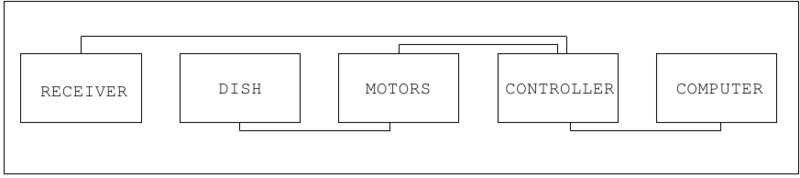
\includegraphics[width=1\textwidth]{block}
  \begin{itemize}
    \item Noise diode allows for calibration of telescope.
    \item Recceiver selects desired bandwidth for data collection.
  \end{itemize}
\end{frame}

\begin{frame}
  \frametitle{Peak in Antenna Readings Signal Hydrogen Density Concentration}
  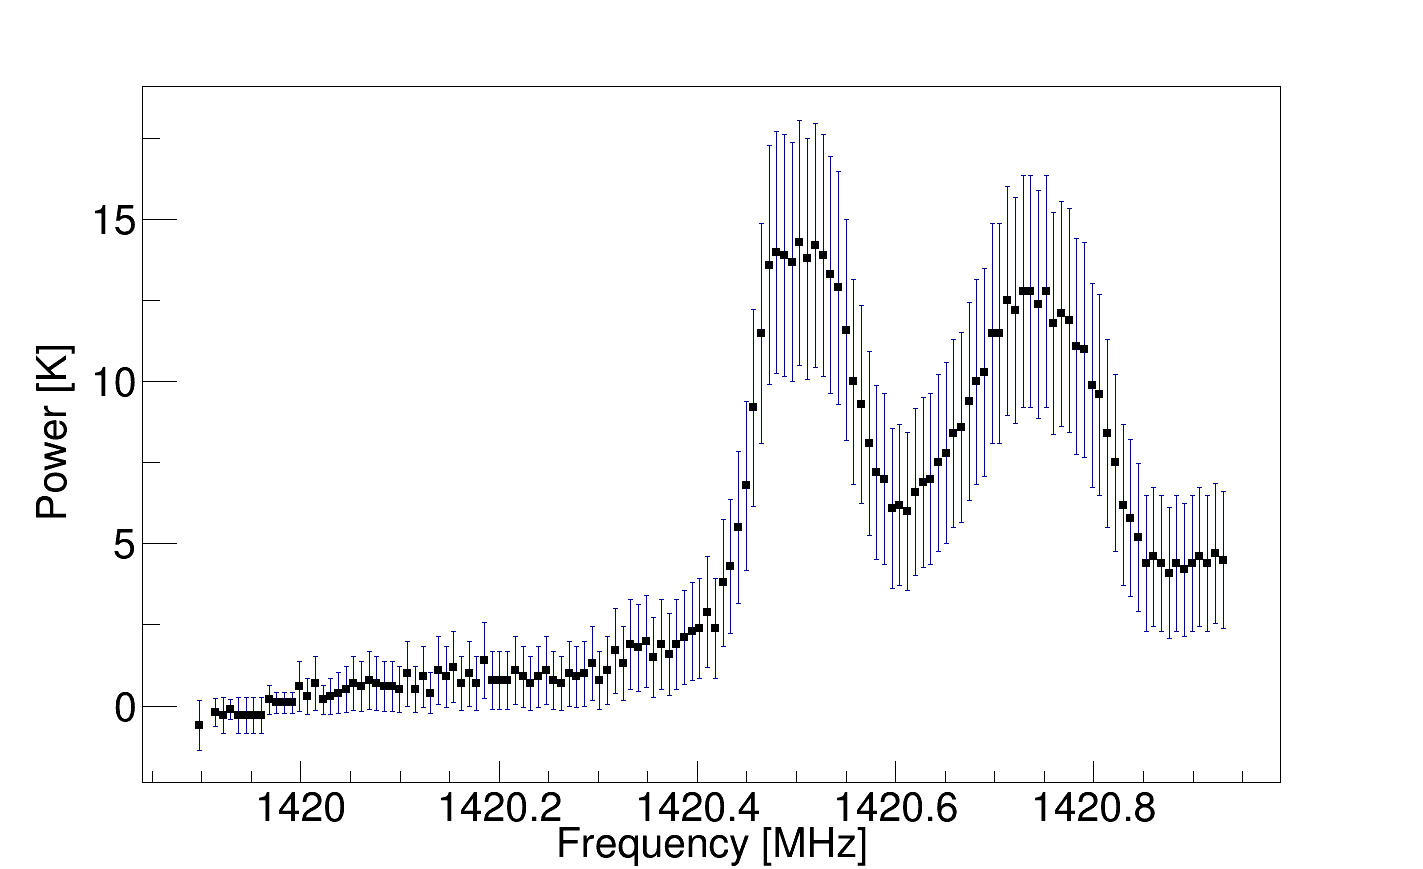
\includegraphics[width=1\textwidth]{data_freq.png}
\end{frame}

\begin{frame}
  \frametitle{Peak in Antenna Readings Signal Hydrogen Density Concentration}
  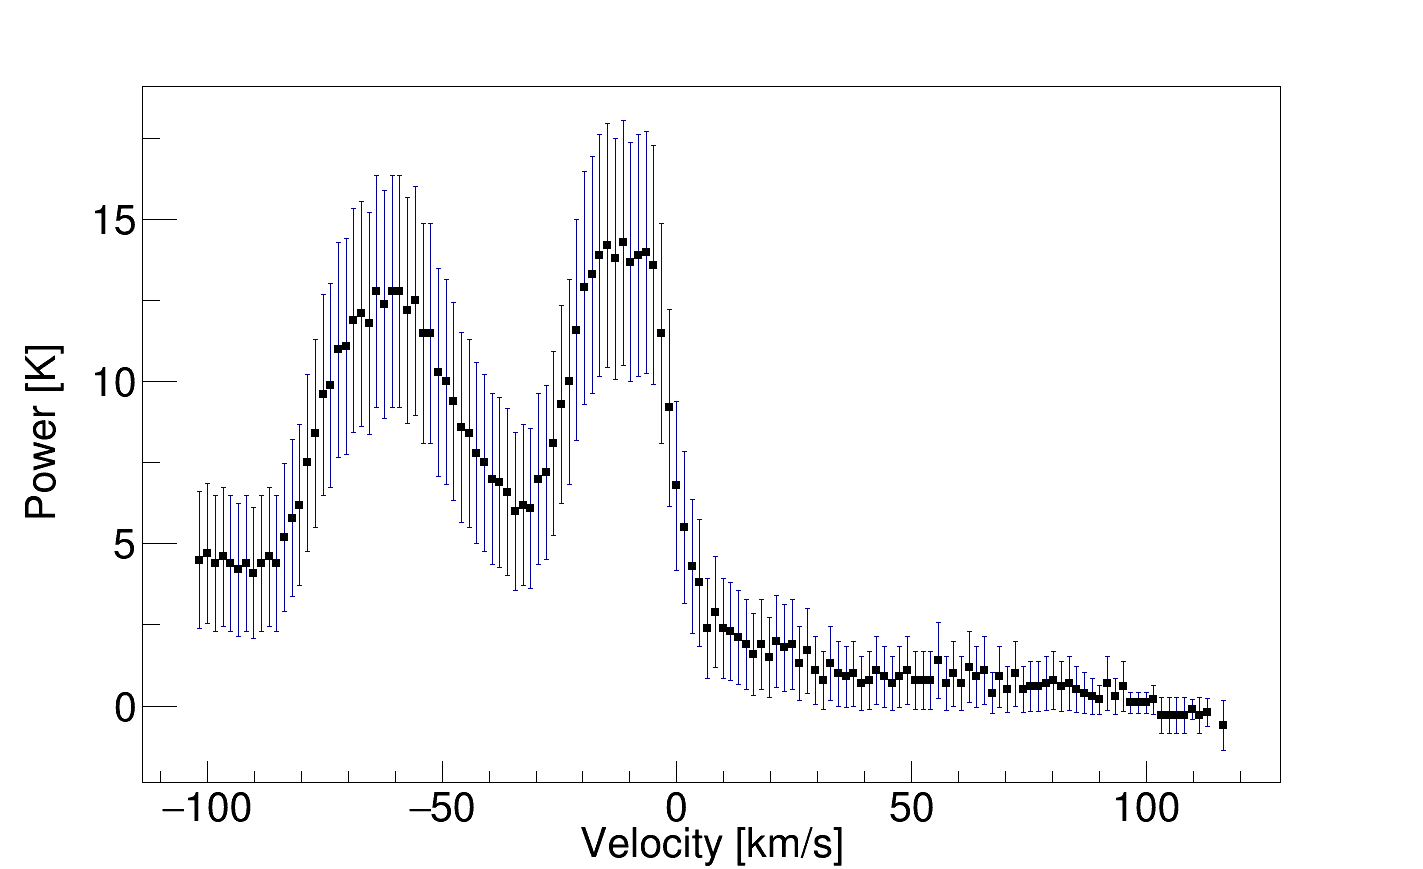
\includegraphics[width=1\textwidth]{data_vel.png}
\end{frame}

\begin{frame}
  \frametitle{Sources of Error Largely Due to Unknown Constants}
  \begin{itemize}
    \item Velocity of sun lacks certainty, approximately $231 \pm 14$ km/s. 
      \pause
    \item Distance from sun to center of galaxy also uncertain, $8.2 \pm 0.5$ kpc. 
      \pause
    \item Poissonian uncertainy in number of counts.
      \pause
    \item Beam width approximated as constant across five degree bin width - taking into account beam profile would allow for more accurate data analysis
  \end{itemize}
\end{frame}

\begin{frame}
  \frametitle{Hydrogen Mapping to Polar Histogram Indicates Spiral Arm}
  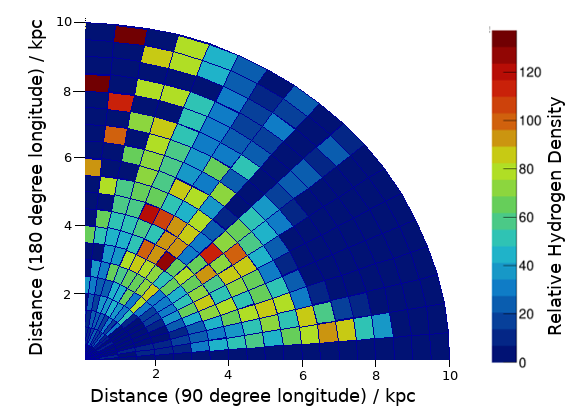
\includegraphics[width=0.8\textwidth]{final.png}
\end{frame}



\end{document}
